\chapter{Peering through the EoR Window}
\label{chapter:eor_window_theory}

Chapter~\ref{chapter:eor_intro} argued the promise of direct observations of {\sc hi} during the EoR. A direct detection has not yet been made, largely due to the overwhelming power of foregrounds compared to the target signal. As shown in Chapter~\ref{chapter:astro_rad}, foreground radiation is a factor of roughly $10^4 - 10^5$ times brighter than predicted 21\,cm anisotropies .  In the past decade, however, enormous improvements have been made in understanding how to decontaminate interferometric visibilities, and excavate the target signal. The leverage astronomers have to use is the exceptional smoothness of low-frequency synchrotron radiation, the dominant foreground emission mechanism. In this Chapter, I review the `Foreground Wedge \& EoR Window' paradigm used to delineate foreground power from noise and {\sc hi} emission. In Section~\ref{sec:eor_window_foreground_wedge} I introduce the concept of the foreground wedge, and methods used by astronomers to take advantage of it: either avoiding it, or subtracting it. In Section~\ref{sec:eor_window_problem_of_pol}, I make plain how astrophysical and instrumental polarization complicates this picture.

\section{Foreground isolation}
\label{sec:eor_window_foreground_wedge}

Mitigation of foregrounds is essential for accessing the EoR. This fact was recognized by \cite{Madau.97} in one of the first in-depth studies of the promises and challenges of 21\,cm tomography. To overcome foreground radiation, they suggested that fitting the synchrotron spectra, relying on its smoothness, may have been sufficiently accurate to subtract the foregrounds from the total signal.
However, for the next two-or-so decades, there were few low-frequency instruments powerful and well-characterized enough to attempt an EoR detection, and precise observations of low-frequency foregrounds did not exist. The first work to concentrate solely on the foreground challenge was \cite{DiMatteo.02}. Their outlook was pessimistic, but they suggested the challenge was surmountable with sufficiently accurate and precise multi-frequency fitting. \cite{Peng.03} were among the first to point out that interferometers are inherently chromatic, and therefore the instrument itself must be taken in to account when considering the frequency dependence of EoR foregrounds.

\cite{Wang.06} were among the first to discover the advantages of describing the foregrounds statistically in Fourier space. Working with numerical simulations, they recognized that forming 1-dimensional power spectra of brightness temperature anisotropies allowed them to isolate the foreground signal to low $k$ values (inverse spatial scales; units h/Mpc), while the EoR signal and noise dominated at high $k$s. With sufficient bandwidth and frequency resolution, one would be able to delineate a boundary between these regions of Fourier space.

Simulating the GSM \citep{GSM.08}, a point source model, and an EoR model transiting a 512-element MWA, \cite{Datta.10} `discovered' the Wedge. They gridded power observed by a baseline in to ($k_{\perp}, k_{\parallel}$) space, where $k_{\perp}$ is proportional to the $u$ coordinate in the $uv$-plane (implying that $k_{\perp}$ is a measure of transverse scales) and $k_{\parallel}$ is proportional to the Fourier-conjugate of frequency (for redshifted 21\,cm emission, a measure of line-of-sight distance). This two-dimensional power spectrum was a generalization of the findings by \cite{Wang.06}, localizing foreground power to low $k_{\parallel}$ values (the `wedge') while 21\,cm power was not as contained, leaving EoR signal and noise at high $k_{\parallel}$ for any given baseline length, proportional to $k_{\perp}$ (see Figure~\ref{fig:eor_theory_wedge_cartoon} for an illustration).

\begin{figure}
\centering
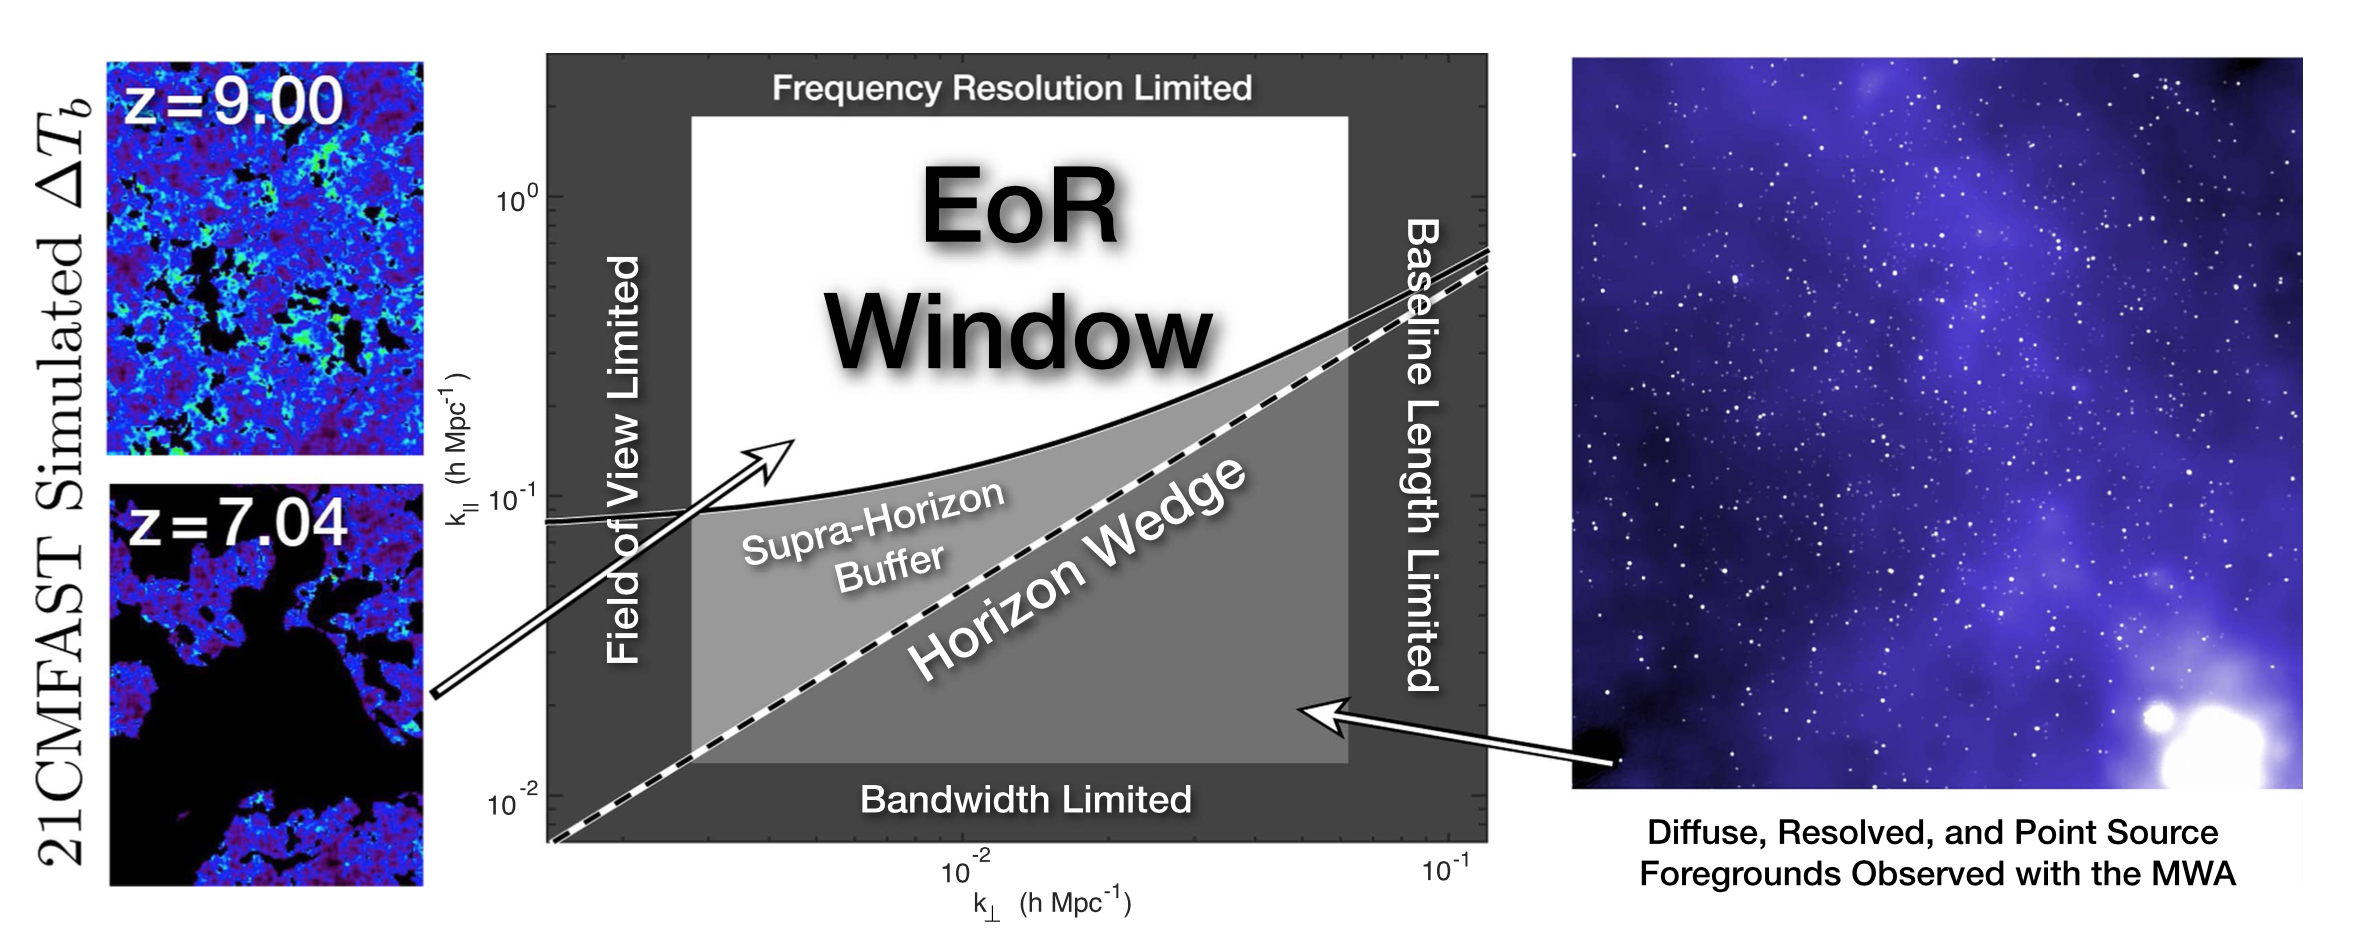
\includegraphics[width=0.8\textwidth]{chapters/eor_window_theory/figures/deBoerWedge.png}
\caption[An illustration of the foreground wedge and the EoR window.]{An illustration of the foreground wedge and the EoR window. Bright synchrotron foregrounds (such as those imaged by the MWA, on the right) are localized in ($k_{\perp}, k_{\parallel}$) to a wedge-shaped region, while spectrally-structured 21\,cm power (simulations from \cite{Mesinger.11} on the left) exists throughout Fourier space -- crucially, outside of the wedge, in an EoR window. \cite{Pober.13} identified the requirement of a buffer region where instrumental effects could spill power just beyond the wedge region. Figure taken from \cite{deBoer.17}.}
\label{fig:eor_theory_wedge_cartoon}
\end{figure}

\cite{Parsons.12a} were the first to provide a quantitative explanation of this structure in Fourier space. In their numerical simulations they recognized that visibilities dominated by smooth synchrotron foregrounds could be Fourier transformed along their frequency axis, and mapped into a narrow region of Fourier space. This is because the sinusoidal structure of the fringe term in the visibility equation, coupled with smooth sky emission and a smooth evolution of the beam term, produced a visibility that could be described with a relatively low number of Fourier modes. However, the inherent spectral structure of 21\,cm emission caused its power to scatter to high $k_{\parallel}$. Crucially, they realized that this allowed per-baseline access to a statistical power spectrum measurement of the EoR.

The wedge \& window paradigm has been continually refined. First-principles derivations from, e.g., \citealt{Trott.12}, \citealt{Vedantham.12}, \citealt{Hazelton.13} and \citealt{Liu.14.1, Liu.14.2} have provided solid theoretical grounding for observational efforts. \cite{Pober.13} identified the requirement of a `supra-horizon buffer' to account for excess power at the boundaries of the wedge, due to a convolution of instrumental spectral structure and beam side-lobes. The buffer is larger for short baselines, since the diffuse structure they probe is typically brighter, and its leaked can dominate over the noise in the EoR window.

\cite{Nithya.15b} identified the importance of the beam for the structure of the EoR window. Forming `pitchfork' (i.e. accounting for the negative Fourier conjugates of frequency; see Figure~\ref{fig:eor_theory_nithya_pitchforks}) power spectra simulations of dipole, phased array and dish-type beams they showed that an identical sky model produced radically different morphologies in Fourier space. Dipole feeds which are capable of observing the entire hemisphere of the sky, such as those used for PAPER, created full `wedges' compared to, for example, dish elements, the tapered response of which isolated power to much narrower regions of Fourier space. Phased arrays, such as those used by the MWA, lay in a middle-ground of sorts. Their findings are reproduced in Figure~\ref{fig:eor_theory_nithya_pitchforks}.

\begin{figure}
\centering
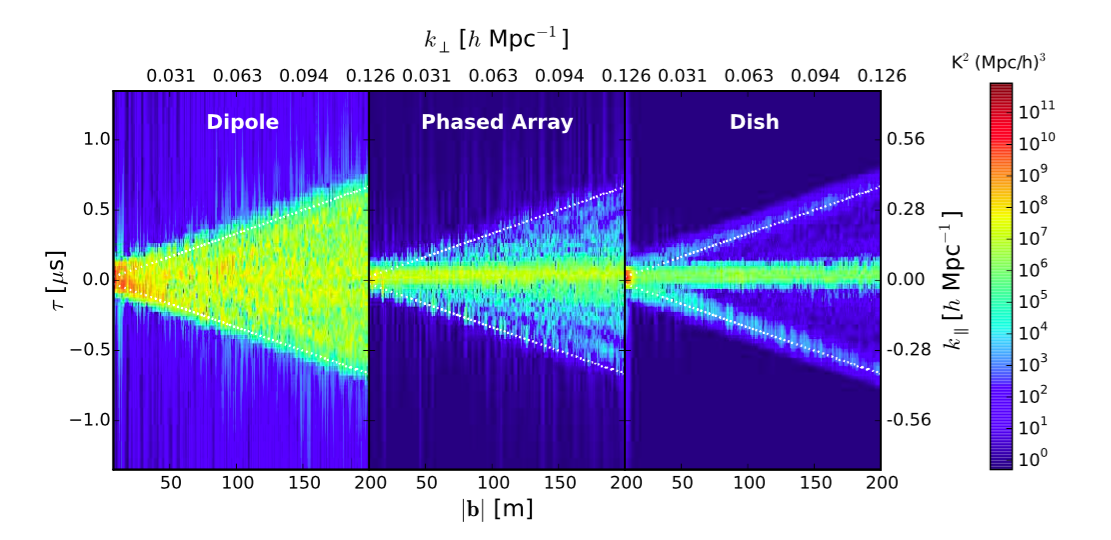
\includegraphics[width=0.8\textwidth]{chapters/eor_window_theory/figures/nithyaWedge.png}
\caption[Different instrument receptivity patterns -- dipoles, phased arrays and dishes -- have different 2D power spectrum morphologies.]{Different instrument receptivity patterns -- dipoles, phased arrays and dishes -- have different 2D power spectrum morphologies. Figure taken from \cite{Nithya.15b}.}
\label{fig:eor_theory_nithya_pitchforks}
\end{figure}

Once the wedge and window have been formed, how does one proceed to extract the 21\,cm EoR signature from the noise? As mentioned above, the instrument used to make the measurement will play a key role in this decision, and PAPER, the MWA and LOFAR have approached extraction of the signal from different directions. These can be roughly placed in to two categories: foreground avoidance and foreground subtraction.

\subsection{Foreground avoidance}

The foreground avoidance strategy is roughly synonymous with the `delay spectrum' approach. \cite{ParsonsBacker.09} defined the delay spectrum as the Fourier transform of a visibility with respect to the frequency axis (c.f. Chapter~\ref{chapter:interferometry}; Section~\ref{subsubsec:interferometry_1dclean}),
\begin{equation}
\tilde{V}_{ij}(\tau,t) = \int {\rm d}\nu V_{ij}(\nu,t)e^{2\pi i \nu \tau},
\end{equation}
for delay $\tau$. This transform maps flat-spectrum emitters to Dirac delta functions in delay space, where the delay of the source is the geometrical time delay for their radiation to be received by antenna $i$ and antenna $j$ (see Figure~\ref{fig:delay_space_parsons12b}). Note that this implies a maximum possible delay value, given by the light travel-time along the baseline vector. This maximum occurs at the horizon, and is referred to as the `horizon delay' or `horizon limit', $\tau_h$. With sufficient bandwidth and frequency resolution, this boundary can be clearly delineated, shown as black dashes lines for baselines of increasing length in Figure~\ref{fig:eor_window_parsons_adapt}. Synchrotron sources are not typically flat-spectrum, but their spectra are smooth. This creates a broadening kernel that convolves the delta function at a given delay. Emission with more frequency structure will have a broader signature in delay space. This is the primary motivation of the delay spectrum. Fourier-transforming foreground emission will contain it at delay values $\tau \leq \tau_h$, whereas spectrally structured EoR and noise power will scatter in to modes $\tau > \tau_h$. Figure~\ref{fig:eor_window_parsons_adapt}, adapted from \cite{Parsons.12a}, illustrates this by simulating the delay spectra of visibilities containing four smooth-spectrum sources and a greatly-amplified EoR signature in one portion of the sky. A Blackman-Harris window was used during the delay transform to minimize sidelobes. Time increases up the vertical axis; as time goes by, sources rise and set from horizon to horizon, but the EoR signature exists both inside and outside of horizon delays. The baseline dependence of the maximum delay foregrounds are allowed to occupy is what gives rise to the pitchfork shown in Figure~\ref{fig:eor_theory_nithya_pitchforks}.

\begin{figure}
\centering
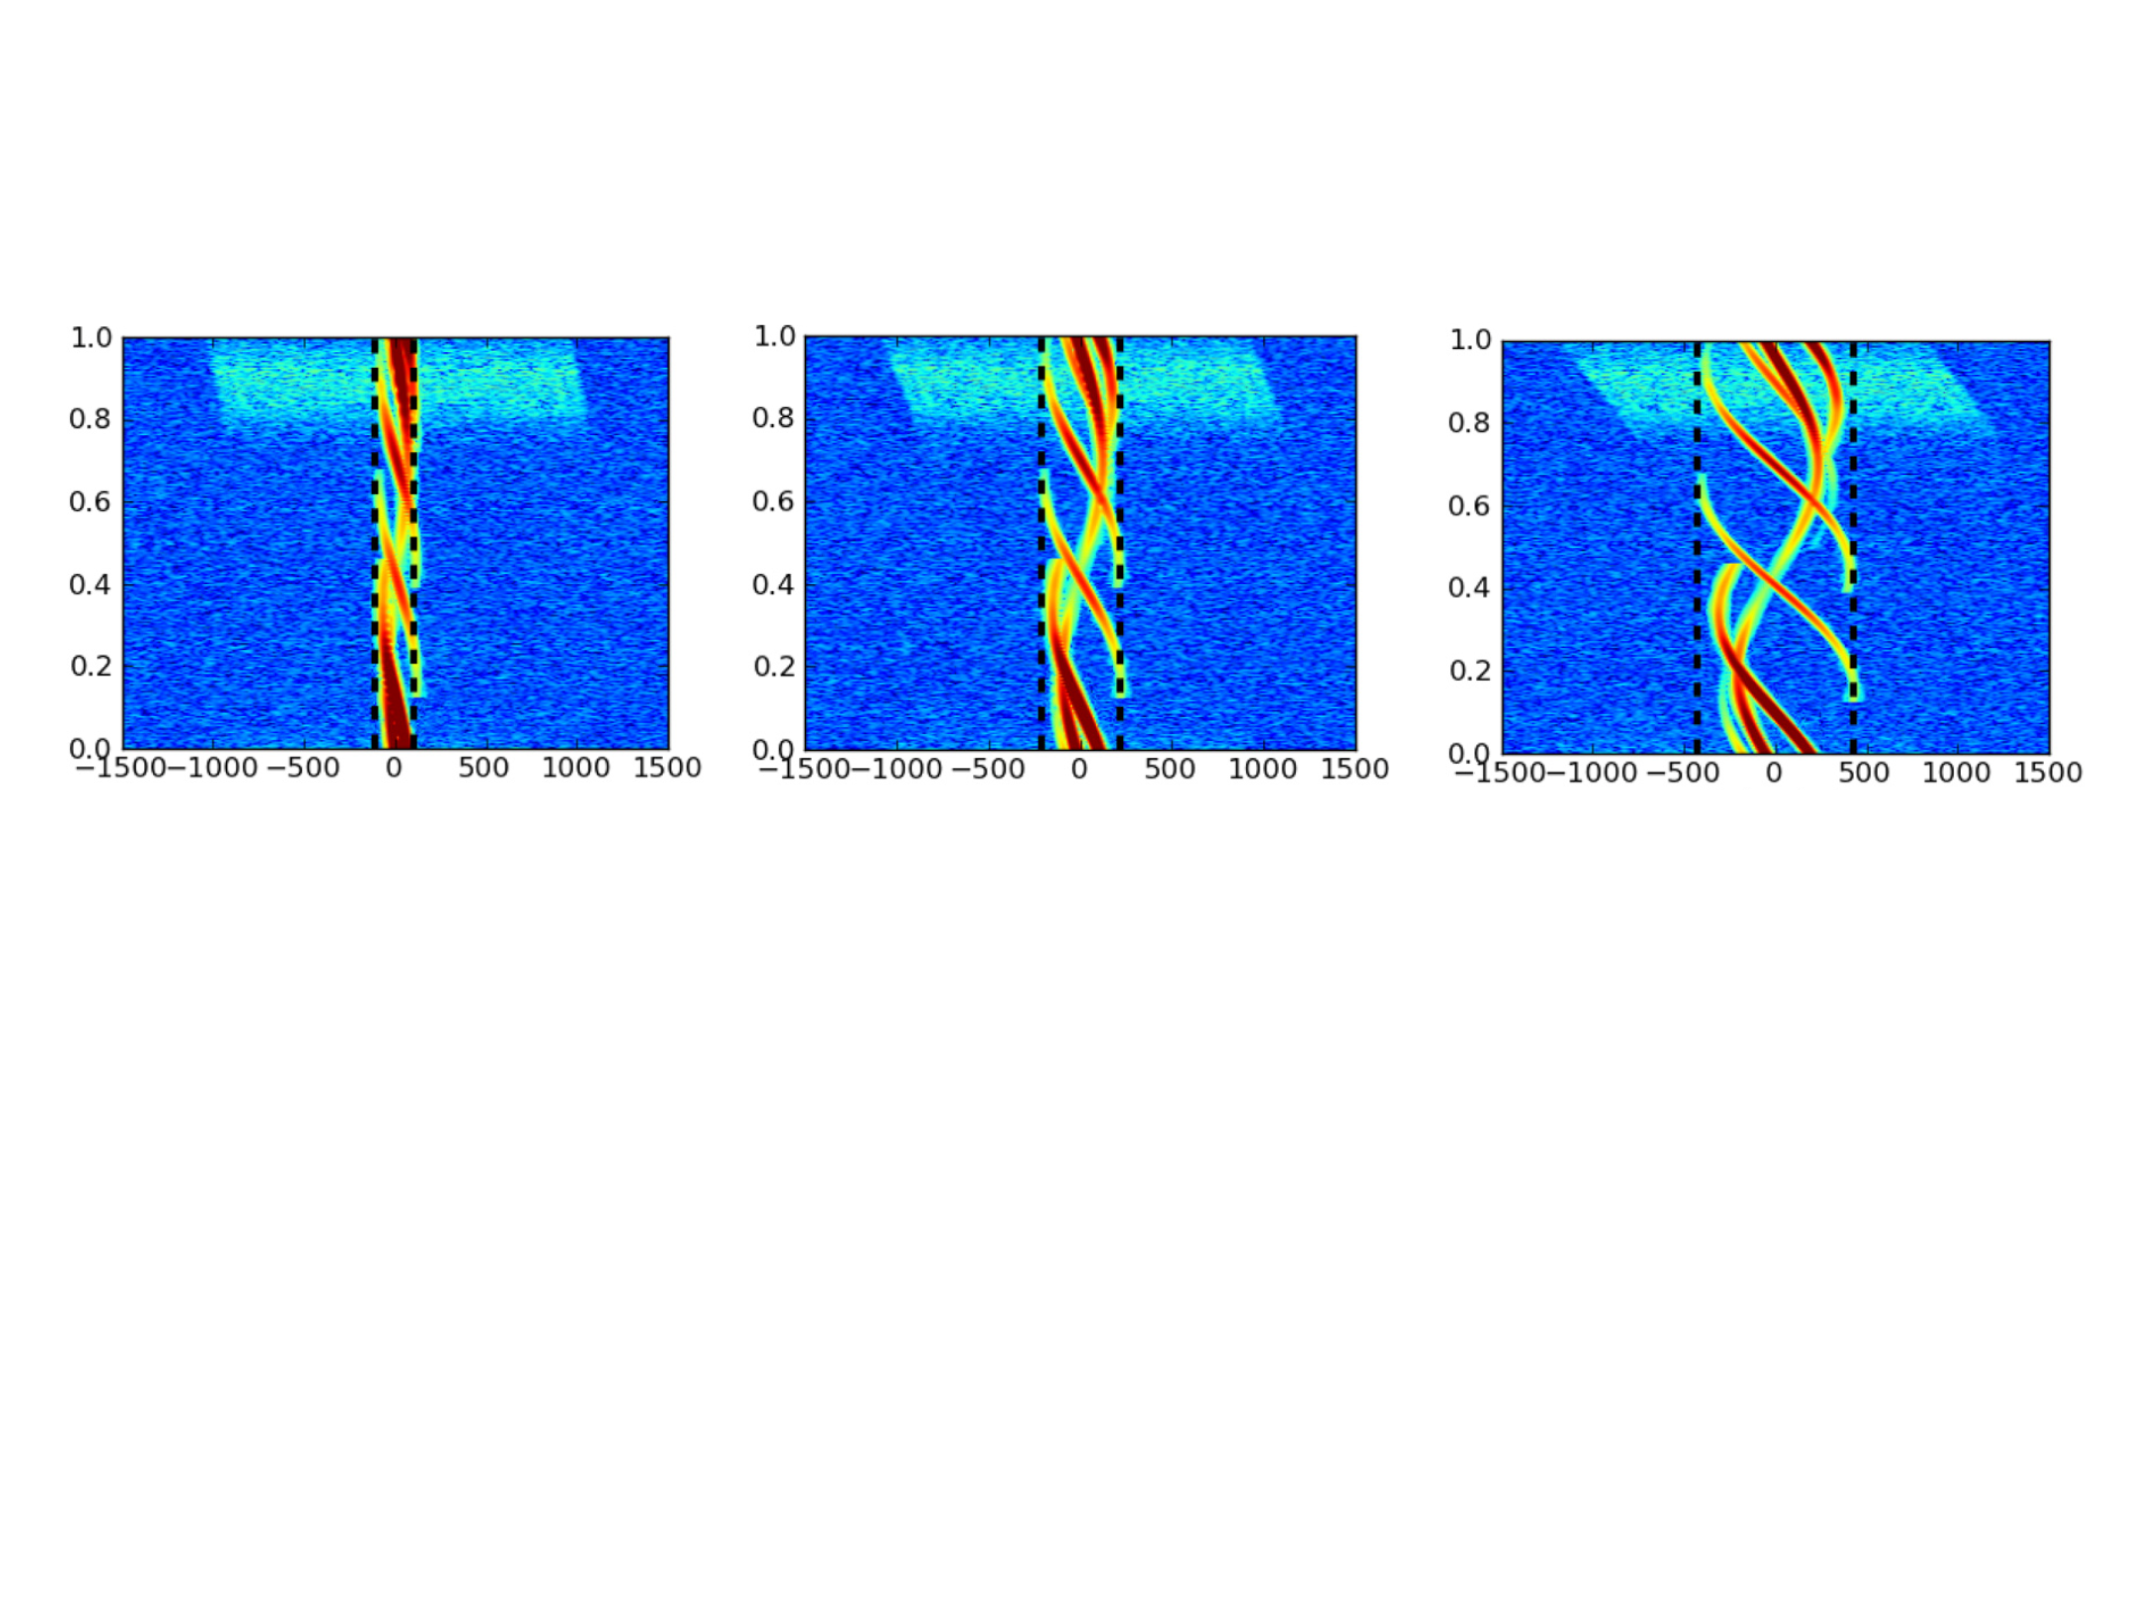
\includegraphics[width=0.9\textwidth]{chapters/eor_window_theory/figures/parsonsAdapt.pdf}
\caption[Delay vs. time for a simple sky model of four foreground-like, smooth-spectrum sources and an EoR-like (but greatly amplified), spectrally structured signal.]{Delay vs. time for a simple sky model of four foreground-like, smooth-spectrum sources and an EoR-like (but greatly amplified), spectrally structured signal. The foregrounds are contained within horizon delays (black dashed lines), but the EoR signal scatters outside of the boundaries. The three panels show the same sky observed by progressively longer baselines (left to right: 32, 64, and 128\,m). The horizontal is in units of nanoseconds, and the vertical axis is in units of days. A Blackman-Harris window was used during the delay transform to minimize sidelobes. Figure adapted from \cite{Parsons.12a}.}
\label{fig:eor_window_parsons_adapt}
\end{figure}

\subsubsection{Power spectra}

To extract cosmological information from observed intensity in delay space, it is useful to form power spectra, which we define for the delay spectrum paradigm below. To convert $u$ to $k_{\perp}$ and $\tau$ to $k_{\parallel}$, \cite{Parsons.12b} defined cosmological scalars:
\begin{align}
X &= 6.5 \times 10^3 \sqrt{\frac{0.27}{\Omega_m}}\left(\frac{1+z}{10}\right)^{0.2} {\,\,\rm h^{-1} Mpc\,rad^{-1}}, \\
Y &= 1.7 \times 10^{-2} \sqrt{\frac{0.27}{\Omega_m}} \sqrt{\frac{1+z}{10}} {\,\,\rm h^{-1} Mpc\,  \,GHz^{-1}},
\end{align}
such that $X$ describes a comoving transverse scale, $Y$ describes a comoving line-of-sight distance, and
\begin{equation}
2\pi(ul + vm + \tau\nu) = k_x x /X + k_y y/ X + k_z z/Y,
\end{equation}
where $l$ and $m$ are directional cosines, $k_i$ measure cosmological wavemodes for comoving coordinates $x,y,z$. $k_z$ and $k_{\parallel}$ are interchangeable in this convention, and $k_{\perp} = \sqrt{k_x^2 + k_y^2}$.

The power measured by a delay-transformed visibility is given by a cross-multiplication of two instances of the visibility. Using the classical visibility equation for simplicity,
\begin{multline}
\tilde{V}^*\tilde{V} \approx \int^{(6)} A(l,m,\nu)A(l',m',\nu') S(l,m,\nu) S(l',m',\nu')\\
					\times e^{-2\pi i (u (l-l') + v (m-m') + \tau (\nu - \nu'))} {\rm d}l {\rm d}l' {\rm d}m {\rm d}m' {\rm d}\nu {\rm d}\nu'.
\end{multline}
We can convert from intensity to brightness temperature using $S(l,m,\nu) = 2k_BT(l,m,\nu)/\lambda^2$. 
This leads to a correlation function $\xi_{T}$ within the integral.
For a beam that spans area $\Omega$ and a delay transform over $\Delta\nu$, \cite{Parsons.12a} showed that the power can be expressed as
\begin{equation}
| \tilde{V}(u,v,\tau) |^2 \approx \frac{\Omega\Delta\nu}{X^2 Y} \left(\frac{2k_B}{\lambda^2}\right)^2 \int^{X\sqrt{\Omega}}_{-X\sqrt{\Omega}} \int^{X\sqrt{\Omega}}_{-X\sqrt{\Omega}} \int^{Y\Delta\nu}_{-Y\Delta\nu} \xi_T (\vec{r})e^{-i\vec{k}\cdot\vec{r}}{\rm d}^3 r.
\end{equation}
In the limit of the integral spanning many phase-wraps of $e^{-i\vec{k}\cdot\vec{r}}$, the integral can be expressed as a power spectrum of $\vec{k}$, and the above equation can be rearranged to give
\begin{equation}
P(\vec{k}) = \left(\frac{\lambda^2}{2k_B}\right)^2 \frac{(\Omega \Delta\nu)^2}{D^2 \Delta D} | \tilde{V}(u,v,\tau) |^2
\label{eq:eor_theory_pspec_def}
\end{equation}
for comoving area $D^2 = X^2\Omega$ and comoving distance $Y\Delta\nu = \Delta D$. For 21\,cm emission, we can describe the transverse and line-of-sight components of $\vec{k}$ as
\begin{equation}
k_{\parallel} = \frac{2\pi\nu_{\rm 21\,cm}H(z)}{c(1+z)^2}\tau ;\,\,\,\,k_{\perp} = \frac{2\pi}{D\lambda}b
\end{equation}

The definition in Equation~\ref{eq:eor_theory_pspec_def} allows us to describe delay-transformed visibilities in terms of cosmological power, as a function of $\vec{k}$. In the foreground avoidance scheme, filters or masks can be implemented to remove or ignore power at values of $k_{\parallel}$ corresponding to delays $\tau \leq \tau_h + \tau_{sh}$, where $\tau_{sh}$ is the supra-horizon buffer discovered by \cite{Pober.13} and chosen by the observer. This nominally leaves only noise and EoR signals in the power spectra.

\subsubsection{Noise spectra}

To estimate the sensitivity of the delay spectrum to 21\,cm anisotropies, we must map the thermal noise of the interferometer in to delay space. Noise in visibilities is described by the \textit{system temperature}, consisting of two components: the receiver temperature ($T_{\rm rxr}$), representing the noise due to the electronics and outside noise from ground reflections and ohmic loss, and the sky temperature ($T_{\rm sky}$), representing the variance in power emitted from the field of observation \citep{TMS}.

Concentrating on the $I\rightarrow I$ component of the direction dependent Mueller matrix (c.f. Chapter~\ref{chapter:interferometry}), 
\begin{equation}
T_{\rm sky}(\nu) = \frac{\int {\rm d}\hat{s} A(\hat{s},\nu) S(\hat{s},\nu) }{\int {\rm d}\hat{s} A(\hat{s},\nu)}
\end{equation}
which at low-frequencies and wide fields-of-view is expected to dominate over $T_{\rm rxr}$. Measuring the average root mean square difference between every-other visibility recorded for a given baseline typically gives a good estimate of the system temperature $T_{\rm sys} = T_{\rm sky} + T_{\rm rxr}$. \cite{Parsons.12b} (and also see public HERA memo \#27) showed that the power spectrum due to system noise is approximately
\begin{equation}
P_N(k) \approx \frac{1}{2\Delta t} X^2 Y \Omega_{\rm eff} B_{\rm NE} T_{\rm sys}^2,
\end{equation}
where $\Delta t$ is the integration time, $B_{\rm NE}$ is the noise-effective bandwidth given by the choice of window used during the delay transform, and $\Omega_{\rm eff}$ is the effective beam area, defined in \cite{Parsons.14} as
\begin{equation}
\Omega_{\rm eff}(\nu) = \frac{| \int {\rm d}\hat{s} A(\hat{s}\nu) |^2}{\int {\rm d}\hat{s} | A(\hat{s},\nu) |^2 }.
\end{equation}

The system temperatures of PAPER and the MWA are between 200 and 300\,K (public HERA memo \#10). These levels make the instrument itself a substantial noise source to overcome in order to reach EoR power levels. This forces EoR experiments to integrate noise down over long observing seasons -- and the data under integration must be noise limited, rather than systematic limited (c.f. Chapter~\ref{chapter:data_prep_and_proc}) -- to obtain limits, and in the future, detections, of the EoR. Cheng et al. (\textit{submitted}) showed in detail that many factors of the observation season contribute to averaging-down the noise. Specifically,
\begin{equation}
P_N(k) \propto \frac{T_{\rm sys}^2}{\sqrt{N_{\rm LST} N_{\rm seps}} t_{\rm int} N_{\rm days} N_{\rm bl} N_{\rm pol}} 
\end{equation}
where $N_{\rm LST}$ are the number of LST hours sampled, $N_{\rm seps}$ are the number of baseline types averaged incoherently (in Chapter~\ref{chapter:eor_window_psa128}, this number is 3),  $t_{\rm int}$ is the effective integration time after fringe-rate filtering (see Chapters~\ref{chapter:data_prep_and_proc} and \ref{chapter:eor_window_psa128}), $N_{\rm days}$ is the effective number of days analyzed, given LST-coverage per day, $N_{\rm bl}$ is the total number of baselines used, and $N_{\rm pol}$ is the number of instrumental polarizations -- which for all power spectra in this thesis is 2.

In Chapter~\ref{chapter:eor_window_psa128} I present the deepest limits achieved by the PAPER experiment using foreground-avoidance techniques. Figure~\ref{fig:eor_intro_pspec_limits} showed the current best limits on the EoR power spectrum, most of which were noise-limited. The best limits still require a factor of $10^3$ more sensitivity before a marginal detection is possible. This in turn requires larger arrays, integrating for longer amounts of time -- an effort that the construction of HERA represents progress on.

\subsection{Foreground subtraction}

Given a finite bandwidth, increasing the length of baselines shrinks the size of the EoR window for that $k_{\perp}$ value. It is possible to construct arrays with such long baselines that the EoR window effectively disappears, and the delay spectrum approach becomes inappropriate. Instead, the wedge must be interacted with in some way. Substantial progress has been made by modelling and subtracting point source contributions from visibilities \citep[e.g.][]{Patil.17}. Point sources dominate the wedge at high $k_{\perp}$ values \citep[e.g.][]{Trott.12} -- subtraction of point source power has the effect of `flattening' the top of the wedge and opening-up some region of it for EoR analysis. However, \cite{Barry.16} showed that an incomplete point source catalog can lead to contamination large enough to prohibit a statistical detection of the EoR.
Both \cite{Kohn.16} and \cite{Patil.17} found -- for very different regions of $k$-space -- that improved phase calibration had a similar effect to point source subtraction, lowering the amplitude of the high ($k_{\perp},k_{\parallel}$) region of the wedge.

\section{The Problem of Polarization}
\label{sec:eor_window_problem_of_pol}

Polarized, Faraday-rotated radiation represents a challenge for both foreground avoidance and subtraction strategies. This challenge is summarized in Figure~\ref{fig:eor_window_theory_pol_problem}. The top panel shows example spectra for various sources of radiation that we are interested in. The largest contribution to overall power observed by our instruments is from Stokes I, where synchrotron emission dominates and emits smooth-spectrum synchrotron. The spectrum of Stokes Q is represented by a $p=1\%$ polarization fraction of Stokes I. The Stokes Q spectrum is also shown Faraday-rotated (see Chapter~\ref{chapter:astro_rad}), and subsequently a fraction $\gamma_{+-}=1\%$ of that Faraday-rotated spectrum can be direction-independently rotated in to Stokes I (see Chapter~\ref{chapter:interferometry}). We choose not to visualize the direction-dependently leaked component as its overall contribution is similar to the direction-independently leaked one. The lower panel shows the delay transform of each spectrum; black dashed lines indicate the horizon delay for a 30\,m baseline.

While Figure~\ref{fig:eor_window_theory_pol_problem} should be considered an illustration, insofar that the absolute values are physically motivated but not precise, its implication is clear. Faraday rotation of polarized foregrounds will, at low frequencies, induce large amounts of spectral structure in the Stokes Q (and Stokes U) spectra. Interferometers can leak power from the Stokes Q and U sky into pseudo-Stokes I visibilities through direction dependent and independent mechanisms -- and this leaked polarized power can represent a foreground with a similar spectral signature to the EoR\footnote{It should also be clear that radio frequency interference from human communications, which manifests as sharp spikes in narrow frequency bands, will have a similar effect to spectrally-structured emission in the delay paradigm.}.

\begin{figure}
\centering
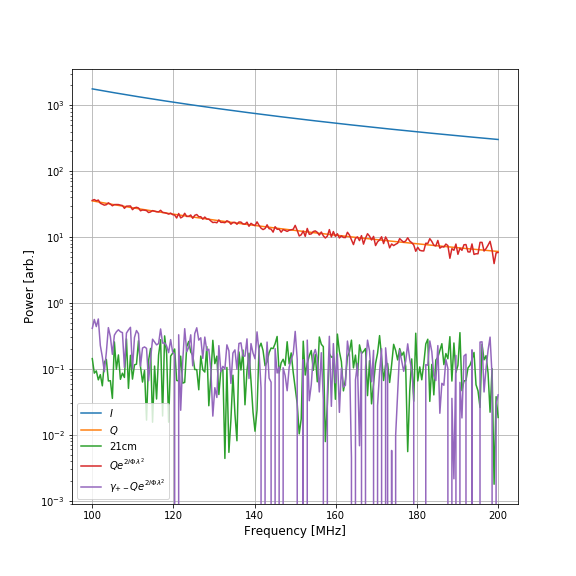
\includegraphics[width=0.55\textwidth]{chapters/eor_window_theory/figures/vis_divBp_1pctDIleak_RM500.png}
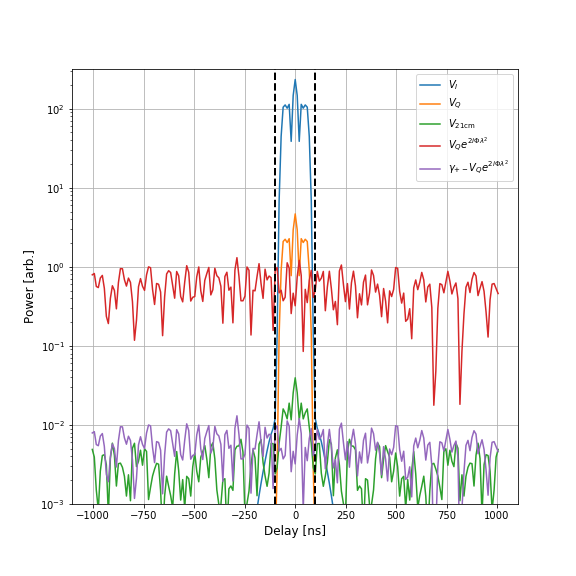
\includegraphics[width=0.55\textwidth]{chapters/eor_window_theory/figures/dly_1pctDIleak_RM500.png}
\caption[A summary of the problem posed by polarization for EoR experiments.]{A summary of the problem posed by polarization for EoR experiments. This is somewhat of a cartoon representation, so the overall power levels should not be taken as accurate forecasts, but they are physically motivated (see Chapter~\ref{chapter:astro_rad}). Above are spectra for unpolarized and polarized synchrotron, the EoR, Faraday-rotated Stokes Q, and a fraction $\gamma_{+-}$ of Faraday-rotated Stokes Q that can leak in to Stokes I. Below, those spectra multiplied by a model bandpass and delay-transformed; the horizon delay for a 30\,m baseline is shown in black. Leaked, Faraday-rotated Stokes Q resembles the EoR.}
\label{fig:eor_window_theory_pol_problem}
\end{figure}

\cite{Moore.13} was the first work to quantify the problem of polarization for the foreground avoidance scheme. Through statistical realizations of the polarized sky, they showed that increasing the average Rotation Measure (RM) contaminated higher $k$ values of the power spectrum. In essence, RMs alias power in the wedge to higher $k_{\parallel}$ values \citep{Nunhokee.17}. Recent measurements have shown that on large scales (low $k_{\perp}$), diffuse emission can be bright, with polarization fractions of 1--4\%, but are observed to have very low rotation measures \citep{Bernardi.13, Lenc.16}. This may mean that polarized power does not represent a large risk to EoR power spectra formed in the foreground avoidance scheme, as leaked power would still remain within the wedge. In the foreground subtraction scheme, one must model each point-source spectrum and subtract it. At the dynamic range required for EoR studies, this necessitates modelling of leaked Faraday-rotated power \citep[e.g.][]{Jelic.14}. Polarized point sources are a greater risk for this approach; \cite{VanEck.18} observed polarized point sources with both high polarization fractions and high rotation measures.

In this Part, I have recorded my efforts to reduce interferometric observations from PAPER and HERA, taking as much care as possible to avoid introducing spectral structure to the visibilities through calibration, and investigating the impact of polarized emission on our measurements. In the following Chapters, I discuss quality assurance metrics and data compression (Chapter~\ref{chapter:data_prep_and_proc}), polarized calibration (Chapter~\ref{chapter:polcal}), the effect of the ionosphere on polarized power spectra (Chapter~\ref{chapter:ionosphere}), and three successively deeper integrations on polarized power, concentrating on successively thinner slices of $k_{\perp}$ (Chapters~\ref{chapter:eor_window_paper32img} -- \ref{chapter:eor_window_psa128}).